\documentclass[10pt,aspectratio=169]{beamer}

%% Paquetes
\usepackage[utf8]{inputenc}
\usepackage[sfdefault,condensed]{roboto}  %% Option 'sfdefault' only if the base font of the document is to be sans serif
\usepackage[T1]{fontenc}
\usepackage[english]{babel}
\usepackage{csquotes}
\usepackage{siunitx}
\sisetup{
    detect-all,
    range-phrase=--,
    range-units=single,
    table-auto-round=true,
    table-format=2.3,
}
\DeclareSIUnit\pixel{px}
\usepackage{booktabs}

\usepackage{tikz} %para la barra de progreso
\usetikzlibrary{calc}

%% Definicion del tema
\useinnertheme{rounded}
\useoutertheme{infolines}
\usecolortheme{orchid}
\setbeamertemplate{navigation symbols}{}


\setbeamersize{text margin left=5mm, text margin right=3mm}

%colores
\definecolor{UVazul}{RGB}{0, 60, 88}
\definecolor{UVazul2}{RGB}{0, 46, 56}
\definecolor{UVturquesa}{RGB}{6, 113, 126}
\setbeamercolor{palette primary}{bg=UVazul,fg=white}
\setbeamercolor{palette secondary}{bg=UVazul2,fg=white}
\setbeamercolor{palette tertiary}{bg=UVturquesa,fg=white}
\setbeamercolor{titlelike}{fg=UVazul2,bg=white}
\setbeamercolor{caption name}{fg=UVazul2, bg=white}
\setbeamercolor{bibliography entry author}{fg=UVazul, bg=white}
\setbeamercolor{bibliography entry note}{fg=UVazul2!80, bg=white}
\setbeamercolor{title}{fg=UVazul, bg=white}
%\setbeamercolor{frametitle}{bg=UVazul2,fg=UVazul}


\makeatletter
% Fuentes
\setbeamerfont{frametitle}{size=\footnotesize,series=\bfseries}
\setbeamerfont{section in head/foot}{size=\footnotesize}
\setbeamerfont{subsection in head/foot}{size=\footnotesize}
\setbeamerfont{title}{size=\Huge,series=\bfseries, shape=\upshape}
\setbeamerfont{author}{size=\normalsize, series=\mdseries, shape=\slshape}
\setbeamerfont{institute}{size=\normalsize, series=\mdseries}
\setbeamerfont{date}{size=\small}
\setbeamerfont{footnote}{size=\scriptsize}

%Titulos 
\setbeamertemplate{frametitle}{} %No apareceran en el frame
\def\insertframetitle{} %Para que no aparezca el titulo en la barra superior

% Params Barra de progreso
\def\progressbar@progressbar{}
\newcount\progressbar@tmpcounta
\newcount\progressbar@tmpcountb
\newdimen\progressbar@pbht
\newdimen\progressbar@pbwd  
\newdimen\progressbar@tmpdim

\progressbar@pbwd=0.35\linewidth
\progressbar@pbht=1.5ex

\def\progressbar@progressbar{%
    \progressbar@tmpcounta=\insertframenumber
    \progressbar@tmpcountb=\inserttotalframenumber
    \progressbar@tmpdim=\progressbar@pbwd
    \multiply\progressbar@tmpdim by \progressbar@tmpcounta
    \divide\progressbar@tmpdim by \progressbar@tmpcountb
    
    \begin{tikzpicture}[rounded corners=2pt, very thin]
        \shade[left color=UVturquesa!50, right color=gray!20] (0pt, 0pt) rectangle ++ (\progressbar@pbwd, \progressbar@pbht);
        \shade[left color=UVazul2, middle color=UVazul, right color=UVturquesa] (0pt, 0pt) rectangle ++ (\progressbar@tmpdim, \progressbar@pbht);
        \draw[color=normal text.fg!50] (0pt, 0pt) rectangle (\progressbar@pbwd, \progressbar@pbht) 
            node[pos=0.5,color=white] {\textnormal{%
                \pgfmathparse{\insertframenumber*100/\inserttotalframenumber}%
                \pgfmathprintnumber[fixed,precision=2]{\pgfmathresult}\,\%%
            }%
        };
    \end{tikzpicture}%
}

%Ventana de titulo
\setbeamertemplate{title page}{
    {%
        \raggedright
        {\usebeamerfont{title}\inserttitle\par}
        \vskip0.35em
        {\color{UVturquesa}\hrule}
        \vskip0.65em
        {\usebeamerfont{author}\insertauthor\par}
        {\usebeamerfont{institute}\insertinstitute\par}
        \medskip
        {\usebeamerfont{date}\insertdate\par}
        \bigskip
    }
    \begin{centering}    
        \inserttitlegraphic\par
    \end{centering}
}


%Barra superior
\setbeamertemplate{headline}{
    \leavevmode%
    \hbox{%
        \begin{beamercolorbox}[wd=.15\paperwidth,ht=3.5ex,right,rightskip=1ex,dp=1.5ex]{section in head/foot}%
            \usebeamerfont{section in head/foot}
            \insertsectionhead
        \end{beamercolorbox}%
        \begin{beamercolorbox}[wd=.25\paperwidth,ht=3.5ex,left,leftskip=1ex,dp=1.5ex]{subsection in head/foot}%
            \usebeamerfont{subsection in head/foot}
            \insertsubsectionhead
            \hspace*{2ex}
        \end{beamercolorbox}%
        \begin{beamercolorbox}[wd=.6\paperwidth,ht=3.5ex,center, dp=1.5ex]{title in head/foot}%
            \usebeamerfont{frametitle}
            \insertframetitle
            \hspace*{2ex}
        \end{beamercolorbox}%
    }%
    \vskip0pt%
}

%Barra inferior
\setbeamertemplate{footline}{
    \leavevmode%
    \hbox{%
        \begin{beamercolorbox}[wd=0.1\paperwidth, ht=2.5ex, right, rightskip=1.5ex, dp=1.5ex]{author in head/foot}%
            \usebeamerfont{author in head/foot}%
            \insertshortauthor%
        \end{beamercolorbox}%
        \begin{beamercolorbox}[wd=.5\paperwidth, ht=2.5ex, left, leftskip=1.5ex, dp=1.5ex]{title in head/foot}%
            \usebeamerfont{title in head/foot}%
            \inserttitle%
            \hspace*{2ex}%
        \end{beamercolorbox}%
        \begin{beamercolorbox}[wd=.4\paperwidth, ht=2.5ex, right, rightskip=2ex, dp=1.5ex]{white}%
            \progressbar@progressbar%
            \vspace*{-1ex}
        \end{beamercolorbox}%
    }%
    \vskip0pt%
}

\makeatother


\usepackage[citestyle=ieee,sorting=nyt]{biblatex}
\addbibresource{bibliografia.bib}

%citas en pie de pagina
\renewcommand*{\bibfont}{\scriptsize}
\newcommand{\citef}[1]{\footnote[frame]{\fullcite{#1}}}
\setlength{\footnotesep}{0.5em}


%% Pagina de titulo

\title[SIPAIM-2023]{A Deep Learning Classifier Using Sliding Patches for Detection of Mammographical Findings}
\author[Mellado et al.]{Diego Mellado, Marvin Querales, Julio Sotelo, Eduardo Godoy, Fabian Pardo, Scarlett Lever, St\'eren Chabert, Rodrigo Salas}
\institute[DCIS-UV]{Doctorado en Ciencias e Ingenier\'ia para la Salud, Universidad de Valpara\'iso}
\titlegraphic{
\includegraphics[height=0.15\textheight]{imagenes/logoUV.png}}
\date{November 16th, 2023}


\begin{document}
    
    {%
        \setbeamertemplate{headline}{}
        \setbeamertemplate{footline}{}
        \begin{frame}
            \titlepage
        \end{frame}
    }%

    \begin{frame}{Acknowledgements}
        This work was funded by:
        \begin{itemize}
            \item National Agency for Research and Development (ANID) / Scholarship program / \textit{Becas Doctorado Nacional 2022} - 21221429
            \item Millenium Science Initiative Program ICN2021\_004
            \item ANID FONDEF IDEA I+D ID20i10332 ``\textit{Artificial Intelligence System for Support in Diagnosis and Priorization of Mammographic Exams}''
            \item ANID FONDECYT Research Grant 1221938
        \end{itemize}

        \begin{figure}
            \centering
            
\includegraphics[height=0.2\textheight]{imagenes/logoIHealth.png}
            
\includegraphics[height=0.2\textheight]{imagenes/logoANID.png}
        \end{figure}
    \end{frame}

    \section{Introduction}
\subsection{Breast Cancer}
\begin{frame}{Breast Cancer in Chile}
    \begin{columns}
        \begin{column}{0.6\textwidth}
            \begin{itemize}
                \item Worldwide, has an average mortality rate of \num{13.6} per \num{100000} women in 2020 \citef{BreastCancerStatistics}
                \item In Chile, has an average mortality rate of \num{11.8} per \num{100000} women, as of 2018 \citef{ministeriodesaludInformeVigilanciaCancer2021}
                \item Early diagnosis and survival rate in Chile has increased due to the implementation of screening programs \citef{castilloResultadosTratamientoCancer2017}
            \end{itemize}
        \end{column}
        \begin{column}{0.4\textwidth}
            \begin{figure}
                \centering
                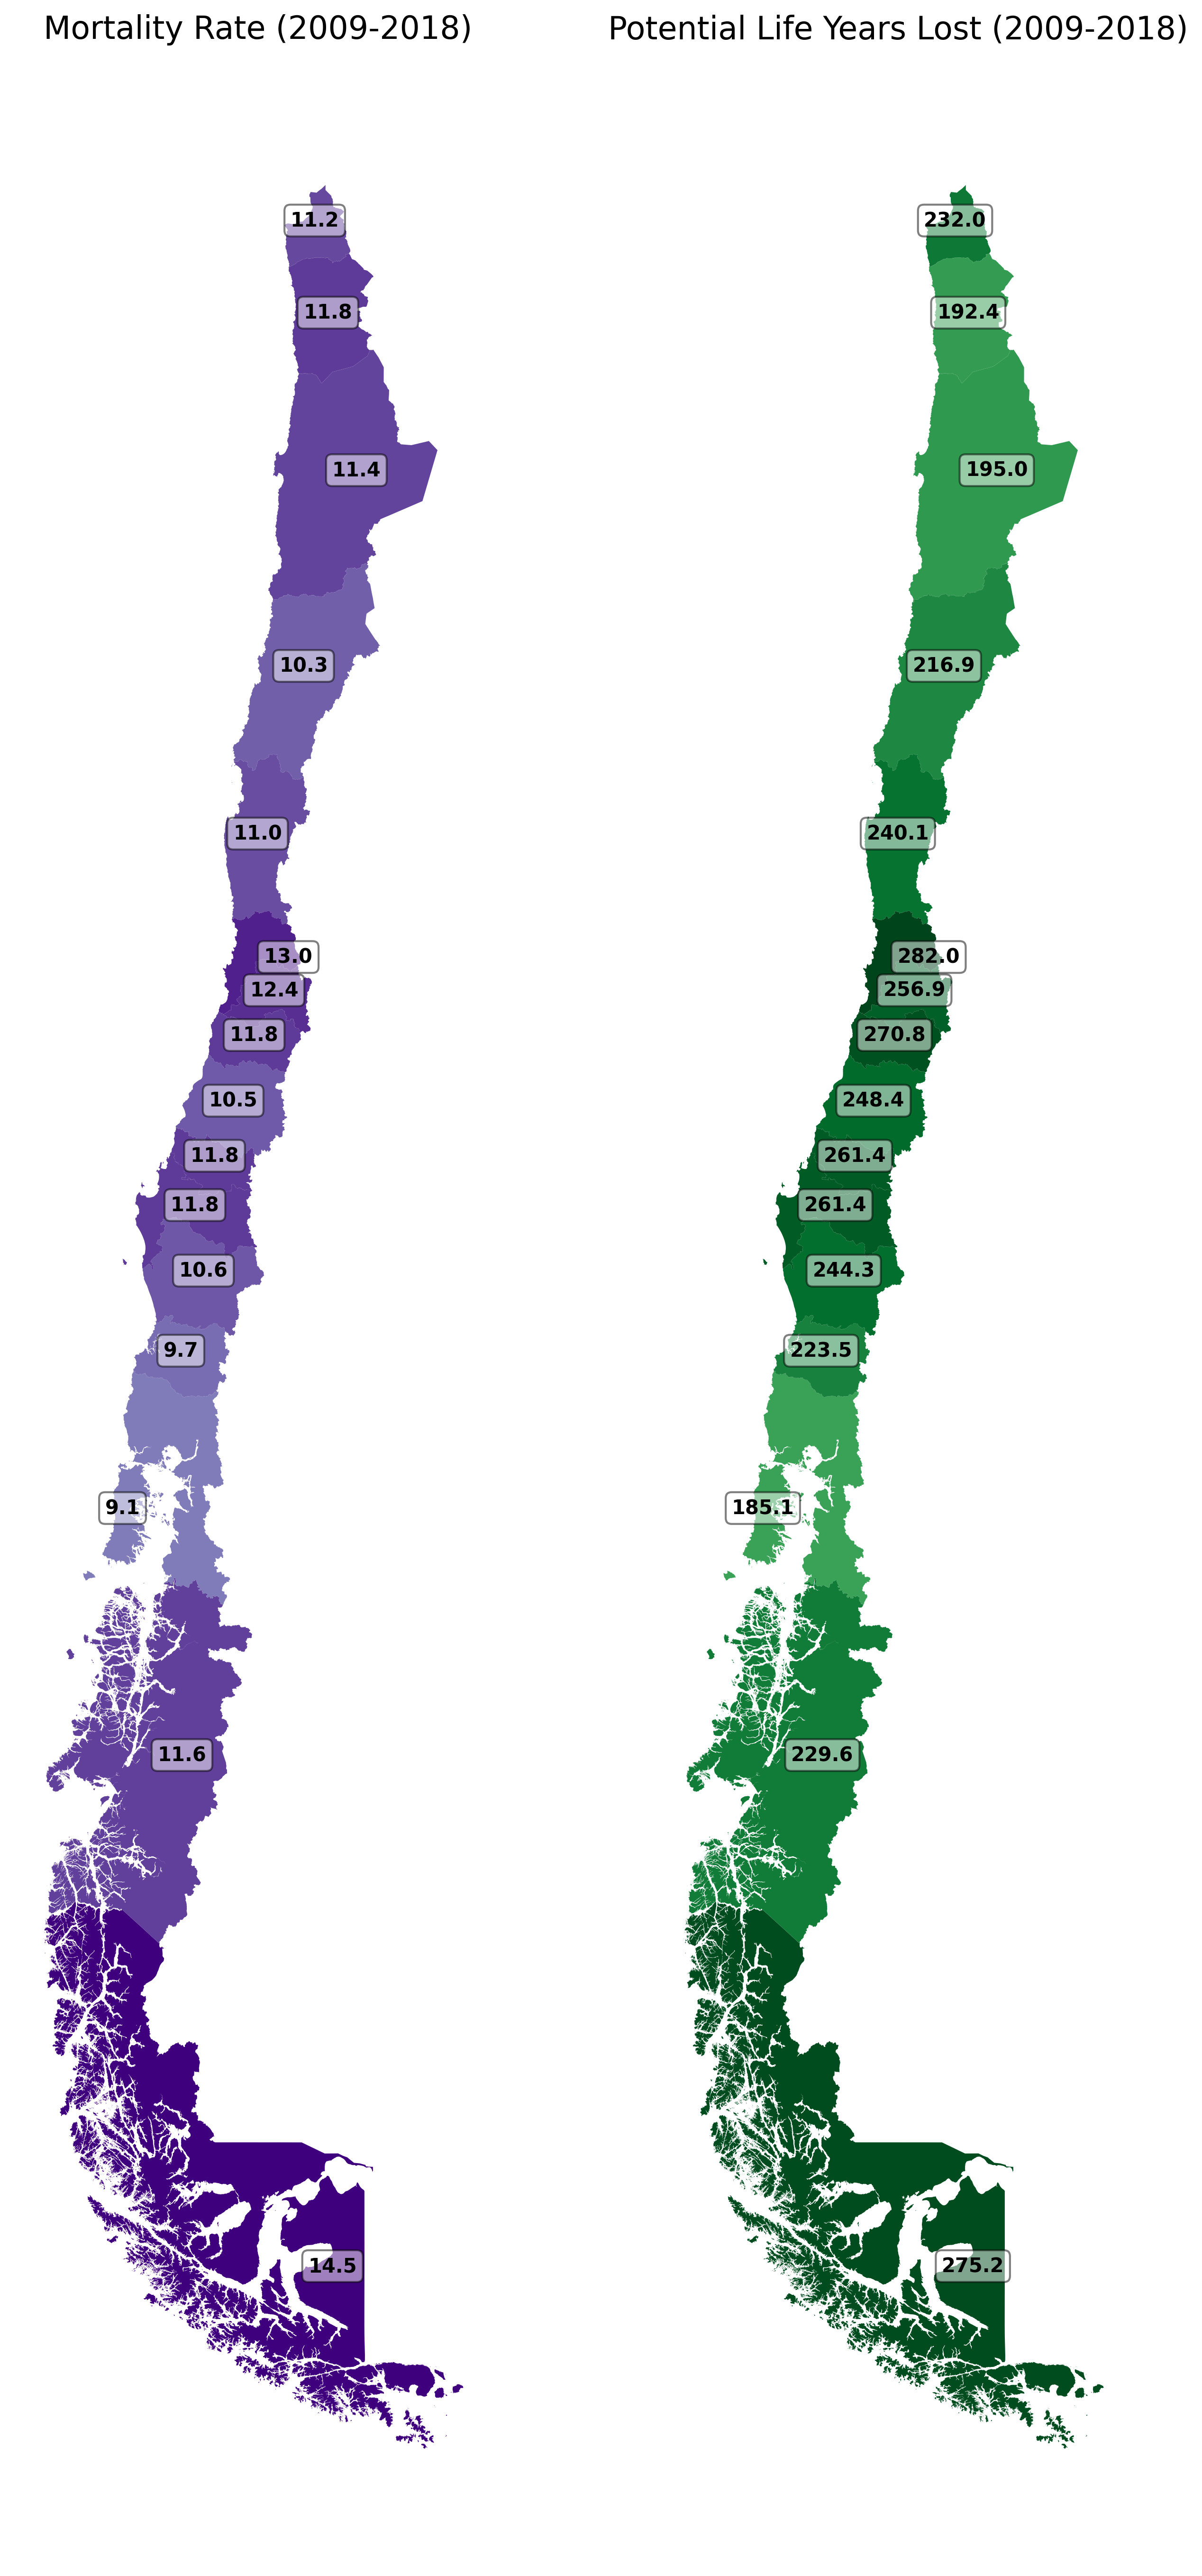
\includegraphics[height=0.5\textheight]{imagenes/mortalidad.png}
                \caption{Mortality rate and number of potential lost years of life due to breast cancer in Chilean Women (2009-2018)}
            \end{figure}
        \end{column}
    \end{columns}
        
\end{frame}

% Descripcion del cancer de mama
\begin{frame}{AI in breast Cancer}
    \begin{itemize}
        \item Machine Learning and Deep Learning models have been implemented for the detection of breast cancer in mammograms. \citef{rodriguez-ruizDetectionBreastCancer2018}
        \item Current Challenges:
        \begin{itemize}
            \item Detection of breast lesion location in mammograms \citef{diazSonSistemasInteligencia2021}
            \item Visualisation tools for interpretation of prediction models.
            \item Breast Density Estimation
            \item Breast image classification beyond malignity.
        \end{itemize}
    \end{itemize}
    
\end{frame}

% metodos de localizar hallazgos
\begin{frame}{Pathological Findings Detection for Breast Cancer}
    \begin{columns}
        \begin{column}{0.3\textwidth}
            \citeauthor{ertosunProbabilisticVisualSearch2015} proposed a Deep Learning model for visual search in mammograms using a regional probabilistic approach. \citef{ertosunProbabilisticVisualSearch2015}

            \begin{figure}
                \centering
                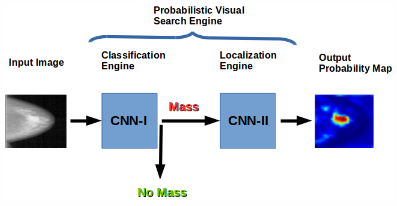
\includegraphics[width=\textwidth]{imagenes/ertosun_probmodel.png}
                \caption{Probabilistic Visual Search Engine proposed by \citeauthor{ertosunProbabilisticVisualSearch2015}}
            \end{figure}
        \end{column}
        \pause
        \begin{column}{0.3\textwidth}
            \citeauthor{frankDeepLearningArchitecture2023}
            proposed using YOLO V5 for detection of breast lesions, combined with EfficientNet for classification of masses and microcalcifications.
            \citef{frankDeepLearningArchitecture2023}

            \begin{figure}
                \centering
                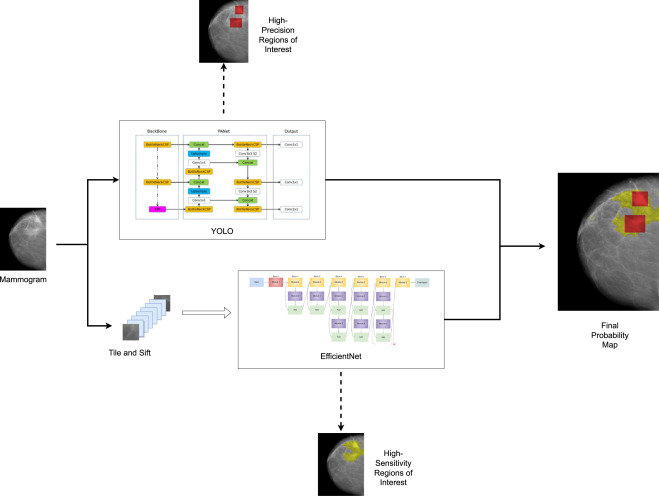
\includegraphics[height=0.3\textheight]{imagenes/frankyolo.jpg}
                \caption{Combined detection model and classifier for breast cancer proposed by \citeauthor{frankDeepLearningArchitecture2023}}
            \end{figure}
        \end{column}
        \pause
        \begin{column}{0.3\textwidth}
            \citeauthor{yiOptimizingVisualizingDeep2017} proposed a model for visualization of shared features between views of the breast for classification of benign and malignant breast tumours.
            \citef{yiOptimizingVisualizingDeep2017}
            \begin{figure}
                \centering
                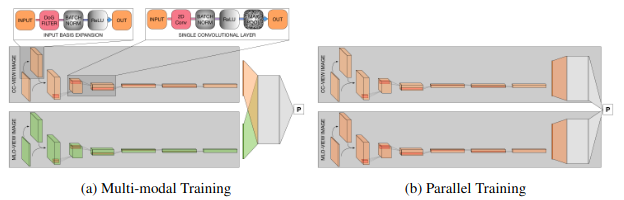
\includegraphics[width=\textwidth]{imagenes/yiparallel.png}
                \caption{Multimodal architecture proposed by \citeauthor{yiOptimizingVisualizingDeep2017} for visualization of shared features between views of the breast.}
            \end{figure}
        \end{column}
    \end{columns}
\end{frame}

% Propuesta del proyecto
\subsection{Proposal}
\begin{frame}{Our Proposal}
    Our study proposes a Deep Learning Classifier trained on cropped segments of mammograms for multi-label classification of pathological findings.

    General Inspection of the complete image using local patches to identify the probability of the presence of a pathological finding.

    \begin{figure}
        \centering
        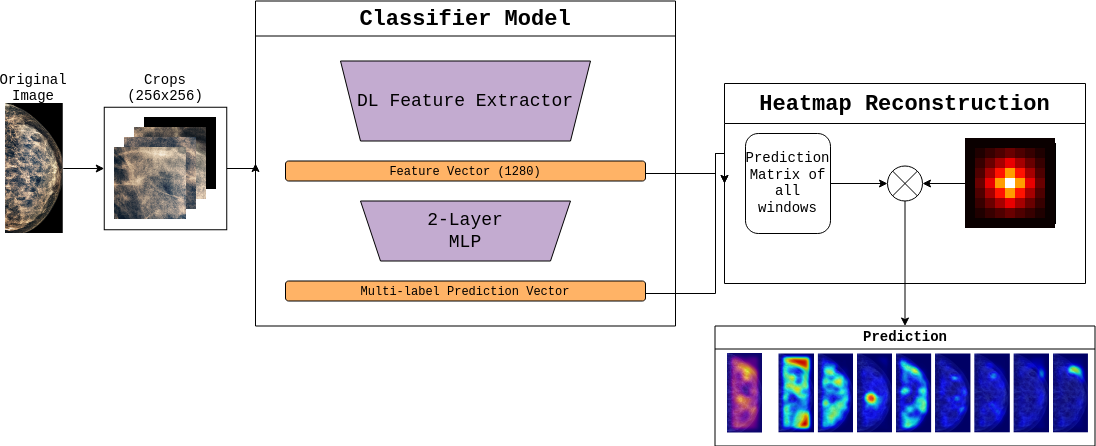
\includegraphics[height=0.5\textheight]{imagenes/modelo.png}
    \end{figure}
\end{frame}


    \section{Methodology}


% Descripcion del dataset
\subsection{Dataset}
\begin{frame}{Dataset}
    \begin{columns}
        \begin{column}{0.5\textwidth}
            \begin{itemize}
                \item \textbf{Vindr-mammo} Dataset \citef{phamhieuhuyVinDrMammoLargescaleBenchmark}
                \item 5000 digital mammogram examinations containing for each view:
                \begin{itemize}
                    \item BIRADs
                    \item Breast density
                    \item Bounding box of each finding present on the image
                \end{itemize}
                \item 10 classes of pathological findings
            \end{itemize}
        \end{column}

        \begin{column}{0.5\textwidth}
            \begin{figure}
                \centering
                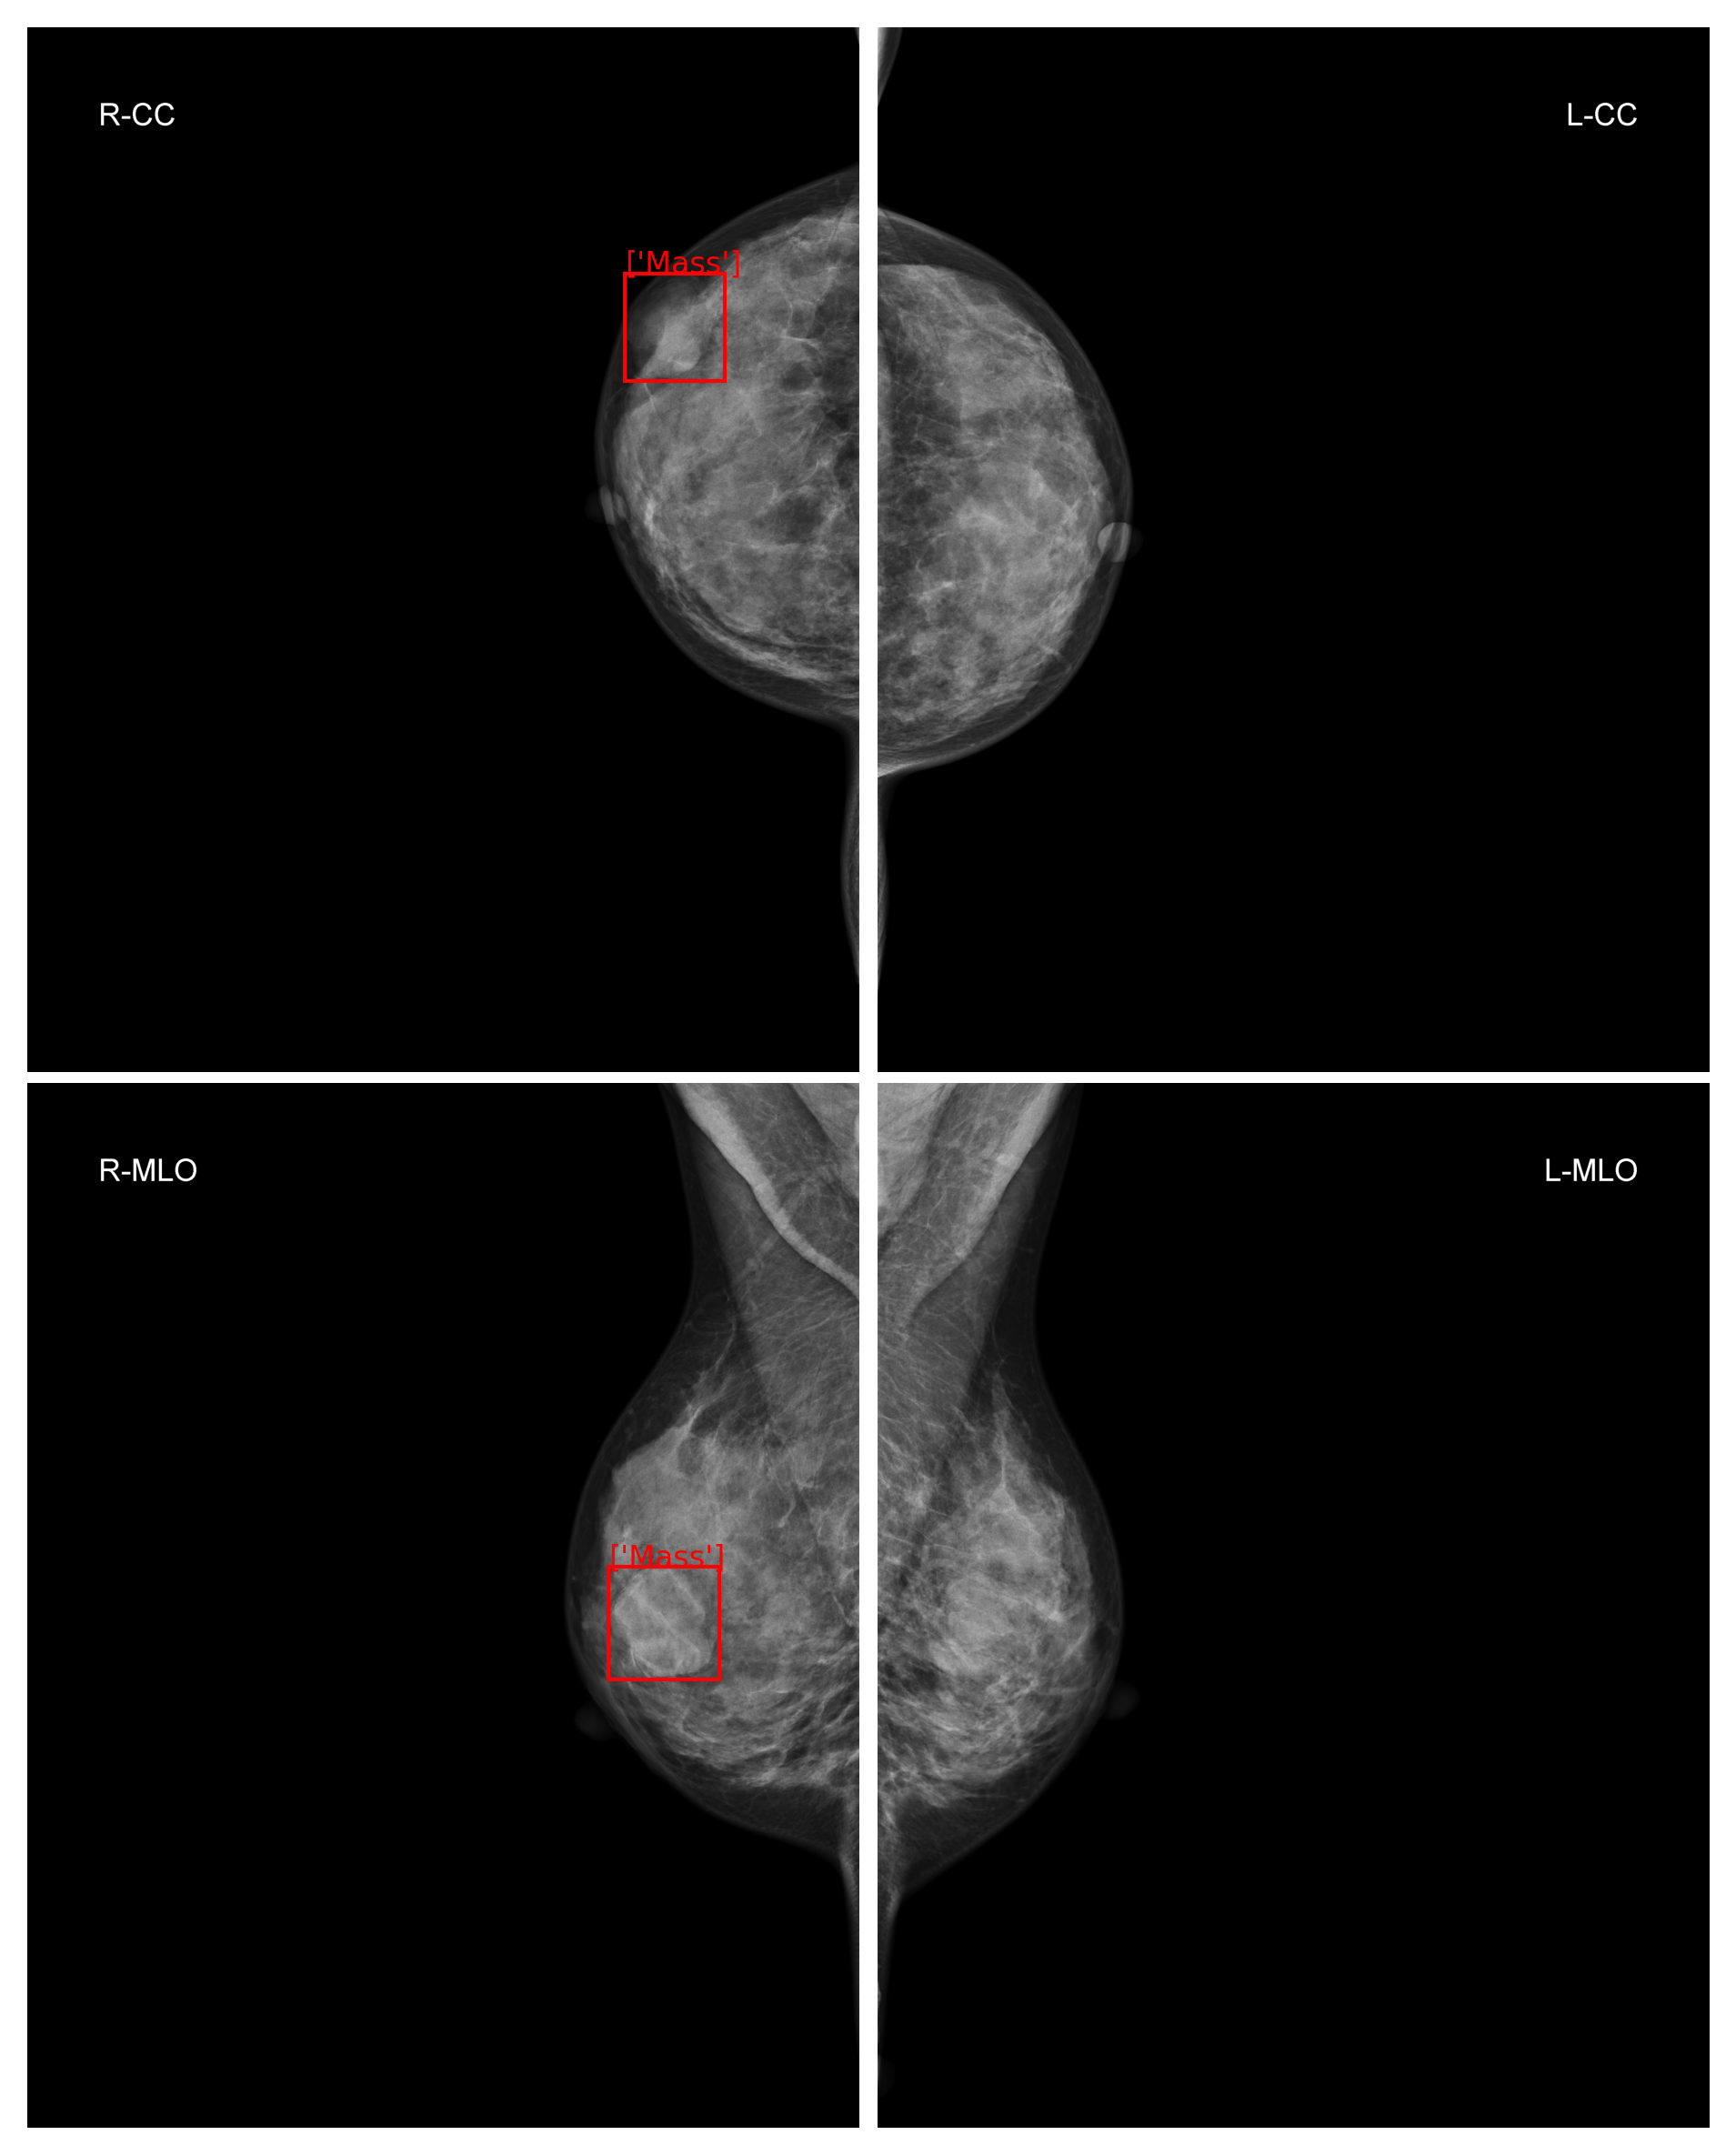
\includegraphics[height=0.5\textheight,keepaspectratio]{imagenes/vista_vindr.png}
                \caption{Example of a mammogram from the Vindr-mammo dataset.}
            \end{figure}
        \end{column}
    \end{columns}
\end{frame}

\begin{frame}{Dataset Distribution}
    
\end{frame}

% Procesamiento de imagenes
\subsection{Image Processing}

\begin{frame}{Image Processing Pipeline}
    \begin{itemize}
        \item Each DICOM Image is normalised to a range of $[0, 1]$
        \item Apply CLAHE algorithm \citef{pizerContrastlimitedAdaptiveHistogram1990} for histogram equalization at 2 different scales
        \item Fuse the equalized images with the original, channel-wise
        \item Image is cropped to the bounding box of the breast using Otsu's thresholding.
    \end{itemize}
\end{frame}

\begin{frame}[plain]
    \begin{figure}
        \centering
        \includegraphics[height=0.9\textheight]{imagenes/improcessingV2.png}
        \caption{Image processing pipeline}
    \end{figure}
\end{frame}
% Seleccion de nuestro modelo
\subsection{Model Selection}
\begin{frame}{Evaluation of deep learning architectures}
    We evaluated the following architectures as a backbone:
    \begin{itemize}
        \item ResNet50
        \item EfficientNetV2
        \item DenseNet
        \item Swin Transformer
        \item MobileNet
        \item VGG19
    \end{itemize}

    Classifier Layer using 2 layer MLP with 512 hidden units and ReLU activation.
    Output layer with 10 units and sigmoid activation.
\end{frame}

% Modelo de extraccion de caracteristicas
\begin{frame}{Feature Extraction Model}
    \begin{itemize}
        \item We use the backbone of the selected architecture as a feature extractor.
        \item The output of the backbone is flattened and fed to the classifier.
        \item The classifier is trained using the cropped images.
    \end{itemize}
\end{frame}

\subsection{Training}
\begin{frame}{Image Sampling}
    \begin{itemize}
        \item For each finding present on an image, we sampled a random area of the finding.
        \item Area and aspect ratio randomly sampled from an Uniform distribution.
        \begin{itemize}
            \item Area: $[.05, 5.]$ of the finding bounding box area.
            \item Aspect ratio: $[0.33 1.66]$ of the finding bounding box aspect ratio.
            \item The bounding box center is uniform sampled from $50$ pixels around the original center.
        \end{itemize}
        \item For normal images (\emph{No Finding}), we sample a random area of the breast, with similar sampling parameters.
        \item Sampled image is resized to $256 \times 256$ pixels.
        \item \textbf{image augmentation}: Contrast, brightness, saturation, flip and rotation are randomly modified.
    \end{itemize}
\end{frame}

\begin{frame}{Training parameters}
    \begin{itemize}
        \item Focal Loss Function 
        \item Adam Optimizer with a starting learning rate of $10^{-4}$
        \item Reduce on plateau with a patience of 5 epochs and a factor of $0.1$
        \item Weighted sampling of the dataset, in order to reduce imbalance.
    \end{itemize}
\end{frame}

% Analisis mediante ventans
\subsection{Sliding patches for detection}
\begin{frame}{Local Information}
    
\end{frame}

\begin{frame}{Our method}
    
\end{frame}

    \section{Results}
\subsection{Model Selection}

\begin{frame}{Results of Model Selection}
    \begin{table}[ht]
\caption{F1 Score for Pathological findings classification task with Vindr, comparing different Deep Learning Models.}
\label{tab:f1score}
\centering
\resizebox{\textwidth}{!}{%
\begin{tabular}{@{}lS[table-format=2]SSSSSS@{}}
\toprule
                         & {N}    & {DenseNet} & {EfficientNet} & {ResNet50} & {SwinTransformer} & {VGG19}   & {MobileNet} \\ \midrule
Mass                     & 237 & 0.7828   & 0.81513      & 0.74163  & 0.76984         & 0.75584 & 0.70833   \\
Suspicious Calcification & 115 & 0.84746  & 0.86463      & 0.85973  & 0.82759         & 0.87288 & 0.82819   \\
Assymetries              & 79  & 0.30645  & 0.29508      & 0.2      & 0.31034         & 0.20370 & 0.32432   \\
Suspicious Lymph Node    & 11  & 0.66667  & 0.5          & 0.73684  & 0.37037         & 0.4     & 0.47619   \\ \midrule
Weighted Average        & 442 & 0.71159  & \bfseries 0.72721 & 0.67543  & 0.69280    & 0.67875 & 0.66511   \\ \bottomrule
\end{tabular}%
}%
\end{table}

    \emph{EfficientNet} has the best overall performance, with an F1 score of \num{0.727}. We chose this model as the backbone for our classifier.
\end{frame}

\subsection{Classifier}
\begin{frame}{Results of our Classifier}
    \begin{columns}
        \begin{column}{0.65\textwidth}
            \begin{table}[ht]
    \centering
    \caption{Metrics of pathological findings classification task using Vindr}
    \resizebox{0.95\textwidth}{!}{%
    \begin{tabular}{p{0.3\textwidth}SSSSS[table-format=4]}
        \toprule
        & {Accuracy} & {Precision} & {Recall} & {F1} & {Support} \\
        \midrule
        No Finding               & 0.9780 & 0.9909 & 0.9844 & 0.9876 & 3643 \\
        Mass                     & 0.9697 & 0.7425 & 0.7300 & \bfseries 0.7362 &  237 \\
        Suspicious Calcification & 0.9902 & 0.8049 & 0.8609 & \bfseries 0.8319 &  115 \\
        Focal Asymmetry          & 0.9834 & 0.2000 & 0.0943 & 0.1282 &   53 \\
        Architectural Distortion & 0.9929 & 0.2222 & 0.0833 & 0.1212 &   24 \\
        Asymmetry                & 0.9951 & 0.0000 & 0.0000 & 0.0000 &   20 \\
        Suspicious Lymph Node    & 0.9978 & 0.6250 & 0.4545 & 0.5263 &   11 \\
        Skin Thickening          & 0.9980 & 1.0000 & 0.3333 & 0.5000 &   12 \\
        Nipple Retraction        & 0.9980 & 0.0000 & 0.0000 & 0.0000 &    7 \\
        Global Asymmetry         & 0.9983 & 0.0000 & 0.0000 & 0.0000 &    6 \\
        Skin Retraction          & 0.9993 & 0.5000 & 0.3333 & 0.4000 &    3 \\
    \bottomrule
    \end{tabular}
    }%
    \label{tab:best_model}
\end{table}
        \end{column}
        \begin{column}{0.35\textwidth}
            Our model achieves a weighted Accuracy of \SI{93.80}{\percent} and a weighted F1 score of \num{0.9557}
        \end{column}
    \end{columns}
    
\end{frame}

\subsection{Sliding patches}
\begin{frame}{Prediction on local windows}
    \begin{figure}
        \centering
        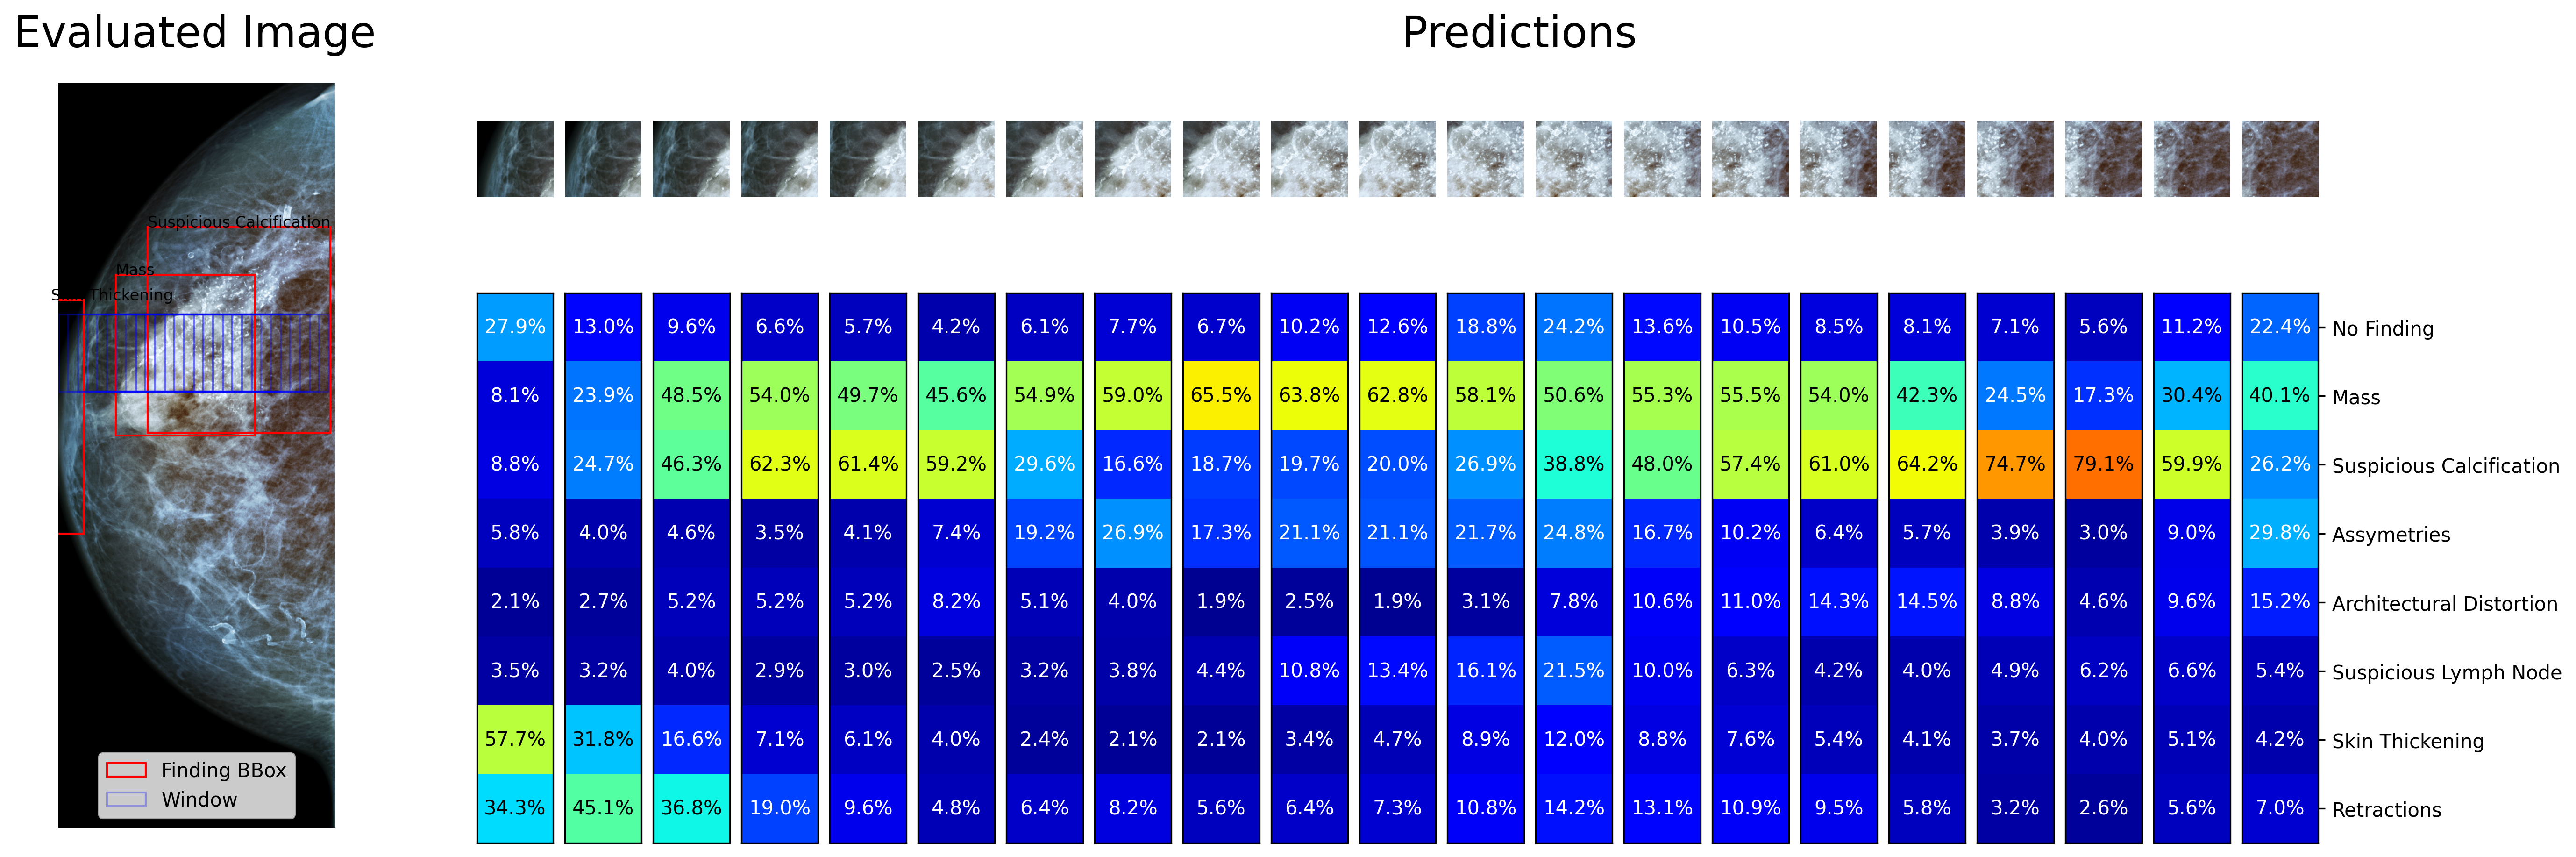
\includegraphics[width=\textwidth]{imagenes/pred_ventanas.png}
        \caption{Image with bounding boxes of its findings and prediction of a row of local windows using our classifier.}
    \end{figure}
\end{frame}

\begin{frame}{Heatmap}
    \begin{figure}
        \centering
        \includegraphics[width=\textwidth]{imagenes/prediction.png}
        \caption{Cropped test image with bounding boxes of its findings, feature activation heatmap, and prediction of the classifier.}
    \end{figure}
\end{frame}

\subsection{Scales}
\begin{frame}{Effects of scale of window}
    \begin{figure}
        \centering
        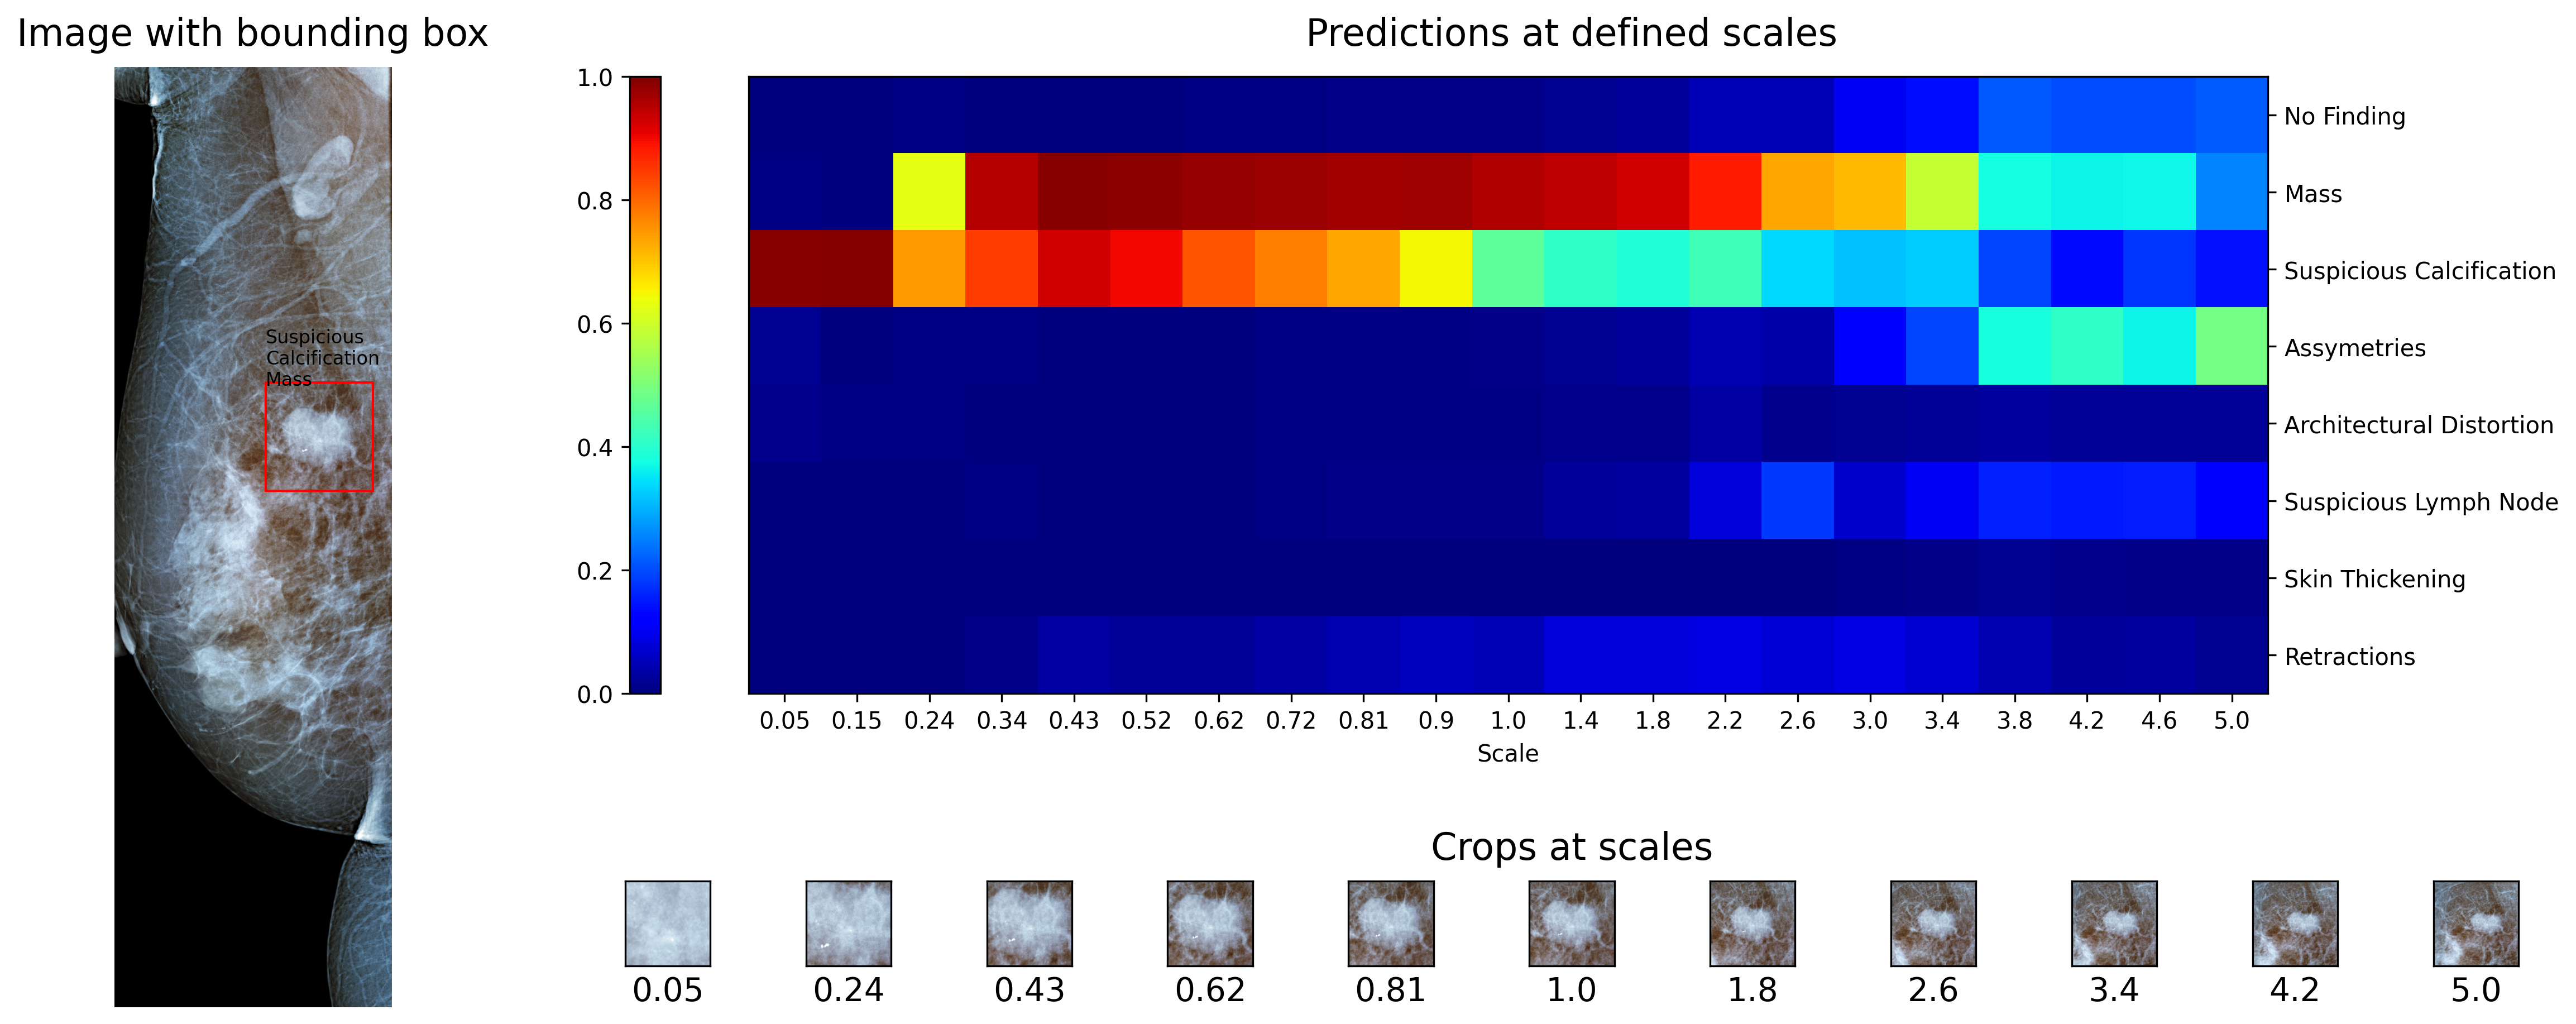
\includegraphics[height=0.7\textheight,keepaspectratio]{imagenes/ratios.png}
        \caption{Prediction of classifier, using finding at different scales.}
    \end{figure}
    
\end{frame}
    \section{Discussion}
\subsection{Discussion}
\begin{frame}{Limitations}
    \begin{itemize}
        \item Low availability of data for some classes impact performance on certain findings.
        \item High sensitivity of the model to the size of findings.
        \item 
    \end{itemize}
\end{frame}

\begin{frame}{Using new data}
    Our model is able to identify findings present in unknown data.
\end{frame}

\begin{frame}{Discussion}
    
\end{frame}

\subsection{Future Work}
\begin{frame}{Future Work}
    
\end{frame}


\end{document}